\chapter{Methods}
This chapter contains a description of the methods used in describing the hardware on the FPGA side using \clash{} and VHDL. The description of the host-side (HPS) programming is included in appendix \ref{app:data_io}, as even though this part of the project is crucial for obtaining results, it is merely tangential to the project goals. 

\section{Overall structure}
In any reasonably complex project it pays off to keep a clear structure: it improves understandability and allows for easier debugging. For simple projects in \clash{}, the structure would be uniquely determined by the HDL generated by \clash{}, but this project also relies on other sources of HDL. Most noteworthy, the interface between the HPS and the FPGA; these signals are very specific to the type of the FPGA and the interconnects it has to the HPS. Luckily, the vendor (Altera) provides a way to generate HDL (the QSys system) in order to create a bridge from the host code running on the HPS to the programmable hardware, the FPGA. This process is described in appendix \ref{app:data_io_setup}. After configuring the bridge, VHDL can be generated and we are left with an instantiable VHDL component. However, even though \clash{} is capable of instantializing external IP components written in VHDL \cite{CLaSHBlogTut}, the most sensible way of implementing such a structure (due to the easy extensibility) is by writing a specific connecting component in VHDL, which can instantiate the \clash{}-generated VHDL. The only responsibility of the connecting component is to distribute and forward signals: it should not perform any computation. It would be a straightforward process of generating such a connecting component based on the signal names in the top-level entities of the components it instantiates, however, due to the fact that it does not change for different designs and it is not very large, the connecting component has been written by hand in VHDL. Figure \ref{f:large_structure} depicts an overview schematic of the complete system, including both the FPGA and HPS side.

\begin{figure}[h]
	\centering
	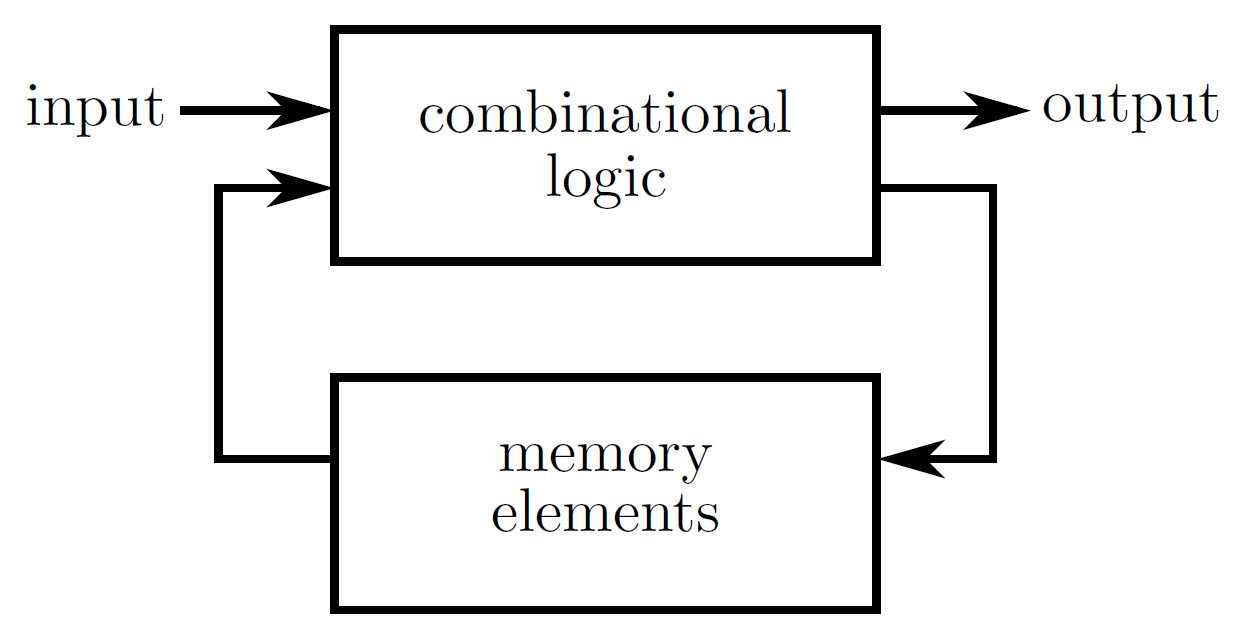
\includegraphics[width=\textwidth]{mealy_machine}
	\caption{TODO ENTER GRAPHIC OF STRUCTURE WITH ILLUSTRATOR}
	\label{f:large_structure}
\end{figure}

\section{External types}
Usually, one of the first things to do when setting up a Haskell project is defining types, and using \clash{} forms no difference. It is especially useful to start by defining an input and an output signal. In a project with simple IO requirements the input and output signals would map straight to switches, keys and LEDs for testing purposes, but as the goal is to write data from the host system into the FPGA registers, the input and output signals will be a lot more complicated. The input and output signals from the \clash{}-generated VHDL top entity are shown in listing \ref{lst:clash_io_types}. The input consists of three separate channels: a bidirectional control channel, the actual input channel and some input needed for the output channel. It might appear strange that the output channel requires input, but this is necessary as the communications adhere to a strict master-slave pattern, in which the HPS is the master and the FPGA the slave. The HPS has to indicate whenever it wants to receive the FPGA output (by specifying an address (\code{out_address}) and setting the \code{out_read}-bit). As a consequence of the strict master-slave protocol, there are a lot less output signals than input signals: only the control and output channel can output data. Lastly, there are the keys, switches and LEDs as additional input and output signals. This concludes the type signatures of the input and output signals in \clash{}-Haskell. However, as the goal is to generate actual VHDL, \clash{} requires some additional information for the naming of the ports of the topEntity of the VHDL module. This is specified using the \code{topEntity}-annotation. In this case this annotation is not very interesting and it's merely a restatement of the input and output signal names, but when the \clash{}-generated VHDL should instantiate other VHDL-modules or use multiple clocks, the annotation can become more complex. It is shown in listing \ref{lst:clash_topentity}. 

\lstinputlisting[caption=Input and output signals for CλaSH, label=lst:clash_io_types, firstline=5,lastline=21]{../clash/SolverTypes.hs}
\lstinputlisting[caption=Signal names\, used in the CλaSH-generated topEntity VHDL module, label=lst:clash_topentity, firstline=8,lastline=29]{../clash/Solver.hs}

\section{Internal types}
So far the external types of the \clash{}-code have been covered, but the real work is done by the internal types: the types that keep track of the state of the system and allow it to do useful work. In order to allow for easy modifications to the types upon which the FPGA operates, they have been defined once and have been referenced everywhere else. This in combination with the property of the higher-order functions in \clash{} that they can operate on all vectors, regardless of length ensures that changing some internal types will not break the program.

\subsection{Internal number representation}
The solvers main data type is \code{type Data = SFixed 8 24}. The constructor \code{SFixed 8 24} stands for a signed fixed-point number, with 8 integer bits and 24 fractional bits. It uses the 2's complement signed number representation, meaning that an 8-bit integer part is capable of representing the integers in the range $[-128..127]$. The 24 fractional bits give this number representation a smallest representable unit of $2^{-24}$. This results in accuracy up to the 7th decimal place, which is similar to the IEEE 754 single precision floating point standard. The main reason for the use of fixed point integers is that \clash{} does not support floating point numbers yet, but additionally, fixed point representations are less demanding on FPGA area and result in a shorter critical path. Furthermore, the reason for choosing the total width of the number representation to be 32-bits is purely convenience: the input and output bridges are also 32 bits wide which allows you to send a single number per write or read.

The \code{UInt} type acts as number representation in cases where only positive integer values are required, for instance in counters.

\lstinputlisting[caption=Internal state variables for CλaSH, label=lst:clash_internal_types, firstline=23,lastline=45]{../clash/SolverTypes.hs}

\subsection{Loading data into the FPGA}
Moving on to the data type which responsible for keeping track of the state of the system: the \code{SystemState}. This type has two fields: the \code{ODEState}, which is has the exact same function as the similarly named type in section \ref{s:numsolHaskell}, it keeps track of the values and the time in the numerical solver. The main difference is that the type of the container containing the actual numerical values of the ODE is not a list. Instead it is a vector. In Haskell, lists can have any length whereas the \clash{}-vectors have a fixed length. This property is very important when generating VHDL, as all vector lengths have to be immutable and known at compile-time in order to change the higher-order functions (eg. map) to hardware. 

In order to understand how the data gets loaded into the FPGA registers it is important to first understand the behaviour of the signals in the input channel originating from the bridge between the HPS and the FPGA. Whenever the HPS program writes the 32-bits value $V$ to 8-bit address $A$, three things happen simultaneously, \code{in_writedata} takes on the value $V$, \code{in_address} gets set to address $A$ and \code{in_write} gets set to true. Only whenever \code{in_write} is true the input value can be considered valid. As the input channel is only used to write initial values to the FPGA, it is sufficient to check whether \code{in_write} has been set to true. If this is the case, the \code{valueVector} of \code{ODEState} in the \code{SystemState} gets updated: the value at \code{in_address} gets replaced with \code{in_writedata}, which gets \code{unpack}'ed into the main data type used by the application. Haskell is a strongly typed language after all, which implies that you cannot simply insert a \code{BitVector 32}, originating from \code{in_write} into a \code{Vec 4 (SFixed 8 24)}. You first have to cast or unpack the \code{BitVector 32} into a \code{SFixed 8 24}, which luckily does not pose any problems as they both consist of 32 bits.

\lstinputlisting[caption=FIX LAYOUT State machine responsible for controlling the solver, label=lst:clash_mealy, firstline=82,lastline=110]{../clash/Solver.hs}

\subsection{Running computations and extracting data}
The \code{step} field takes a bit more explanation. Every time the integration scheme gets applied, the \code{step} variable gets incremented. At some point, the value of \code{step} becomes larger or equal than the \code{maxstep} field from the data type \code{SystemConstants}. Whenever this happens, the system blocks until you order it to start again by setting the value of \code{step} to 0. During the time that the system does not progress, you can read out the values of the system.


\subsection{Implementation of the integration schemes}

\subsection{Implementation of the equations}





